  Dieses Kapitel zeigt Methoden zur Entscheidungsfindung bei einer Evaluation
  auf. Dabei werden die Methoden der gewichteten Nutzwertanalyse und des
  \ac{AHP} gezeigt. Es existieren wahrscheinlich noch weitere Ansätze, welche
  hier nicht behandelt werden.
  
  \section{Grundlagen}
  
  Es gibt verschiedene Methoden wie man bei der Auswahl einer Softwarelösung
  vorgehen kann. Um eine möglichst objektive Betrachtung zu gewährleisten, wurde
  die Methode der gewichteten \ac{NWA} gewählt, siehe \cite{Nutzwertanalyse}.
  Diese Methode stammt aus dem Bereich der quantitativen Analysemethoden der
  Eintscheidungstheorie. Um eine möglichst präzise objektive Gewichtung der
  einzelnen Faktoren zu erhalten wurde dafür die Methode \ac{AHP} gewählt,
  siehe \cite{AnalyticHierarchyProcess}. Diese Methode stammt aus dem Bereich
  der präskriptiven Entscheidungstheorie. Der \ac{AHP} wurde von Thomas L.
  Saaty in den 70er Jahren des 20. Jahrhunderts entwickelt und im Buch ``The
  Analytic Hierarchy Process: Planning, Priority Setting, Resource
  Allocation'', siehe \cite{AnalyticHierarchyProcessBook}, veröffentlicht.
  
  \section{Gewichtete Nutzwertanalyse}
  
  Bei der gewichteten \ac{NWA} wird eine Menge von Alternativen \(\{A1, A2,
  A3, \ldots\}\), auf deren Nutzen, miteinander verglichen.
  
  Als Rahmenbedingung für die Durchführung der Nutzwertanalyse werden \(m\)
  KO-Kriterien \(\{KO_1, KO_2, KO_3, \ldots, KO_m\}\) bestimmt. Ein
  KO-Kriterium wird definiert durch die Erfüllung einer Bedingung. Wenn die Bedingung
  zutrifft, führt das zum KO\footnote{Der Begriff KO steht für Knock-Out und
  stammt aus der Boxwelt. Im falle einer Nutzwertanalyse bedeutet es, dass die
  Alternative aus der Nutzwertanalyse ausgeschlossen wird.} einer darauf
  geprüften Alternative.
  
  Für den Vergleich der Alternativen werden \(n\) vergleichbare
  Soll-Kriterien, auch Anforderungen genannt, definiert \(\{Soll_1, Soll_2,
  Soll_3, \ldots, Soll_n\}\). Jedes Soll-Kriterium wird durch einen
  Gewichtungsfaktor \(g_i\) versehen, was die Präferenz des Soll-Kriteriums
  wiederspiegelt. 

  Die Gewichte \(g_i\) werden so gewählt, dass ihre Summe 1.0 (100\%) ergibt,
  siehe Formel \ref{eq:gewicht}.
  
  Für jede zu evaluierende Alternative soll nun geprüft werden, ob eines
  der KO-Kriterien erfüllt ist, was zu einem Ausschluss der Alternative führen
  würde, siehe Abbildung \ref{img:rahmenbedingungenPruefen}.
  
  Falls das nicht für alle Alternativen der Fall ist, wird ein Vergleich der
  im Rennen bleibenden Alternativen über die definierten Soll-Kriterien
  geführt. Dabei werden für jede Alternative die einzelnen Soll-Kriterien mit
  einem Erfüllungsgrad \(e_i\) bewertet. Die Skala der Erfüllungsgrade ist in
  der Tabelle \ref{tab:erfuellungsgrade} ersichtlich.
  
  Der Nutzwert einer Alternative ergibt sich durch die Formel \ref{eq:nutzwert}.
  \newline
  
  \begin{table}[hbt]
    \sffamily 
    \begin{center}
      \begin{tabular}{lc}
        \toprule
        \textbf{Erfüllungsgrad} & \textbf{Skala}\\
        \midrule
        nicht erfüllt & 0\\
        schlecht & 1, 2\\
        mittel & 3 - 5\\
        gut & 6 - 8\\
        sehr gut & 9\\
        \bottomrule
      \end{tabular}
      \caption{Skala der Erfüllungsgrade}
      \label{tab:erfuellungsgrade}
    \end{center}
  \end{table}
  
  Diejenige Alternative mit dem grössten Nutzwert entspricht am meisten den
  Anforderungen. Wie gut eine Alternative nun den gestellten Anforderungen
  entspricht, kann anhand ihres berechneten Nutzwertes in der Tabelle
  \ref{tab:erfuellungsgrade} abgelesen werden.

  \begin{equation}
    \label{eq:gewicht}
    Gewicht := \sum \limits_{i=1}^n g_i = 1.0
  \end{equation}
  
  \begin{equation}
    \label{eq:nutzwert}
    Nutzwert := \sum \limits_{i=1}^n e_i \cdot g_i
  \end{equation}
  
  \subsection{Anschauliches Beispiel}
  
  Als anschauliches Beispiel sollen zwei Alternativen - Auto \(A1\) und Auto
  \(A2\) - miteinander auf die Soll-Kriterien - Leistung, Aussehen und
  Alltagstaublichkeit - verglichen werden. Es wurden keine KO-Kriterien
  definiert. In der Tabelle \ref{tab:beispielNwa} ist ersichtlich, dass das
  Auto \(A1\) dem Auto \(A2\) gegenüber bevorzugt werden soll, da der Nutzwert
  von \(A1\) (5.0) grösser ist als der Nutzwert von \(A2\) (4.7).
  \newline
  
  \begin{table}[h!]
    \sffamily 
    \begin{center}
      \begin{tabular}{lrrrrr}
        \toprule
        \textbf{Kriterien} & \textbf{Gewichtung \(g\)} & \textbf{\(e_{A1}\)} &
        \textbf{Wertigkeit \(A1\)} & \textbf{\(e_{A2}\)} & \textbf{Wertigkeit
        \(A2\)}\\
        \midrule
        Leistung            & 0.3 & 7 & 2.1 & 9 & 2.7 \\
        Aussehen            & 0.2 & 2 & 0.4 & 5 & 1.0 \\
        Alltagstauglichkeit & 0.5 & 5 & 2.5 & 2 & 1.0 \\
        \midrule
        \midrule
        Ergebnis            & 1.0 &   & 5.0 &   & 4.7 \\
        \bottomrule
      \end{tabular}
      \caption{Beispiel einer Nutzwertanalyse}
      \label{tab:beispielNwa}
    \end{center}
  \end{table}
  
  \begin{figure}[htb]
    \begin{center}
      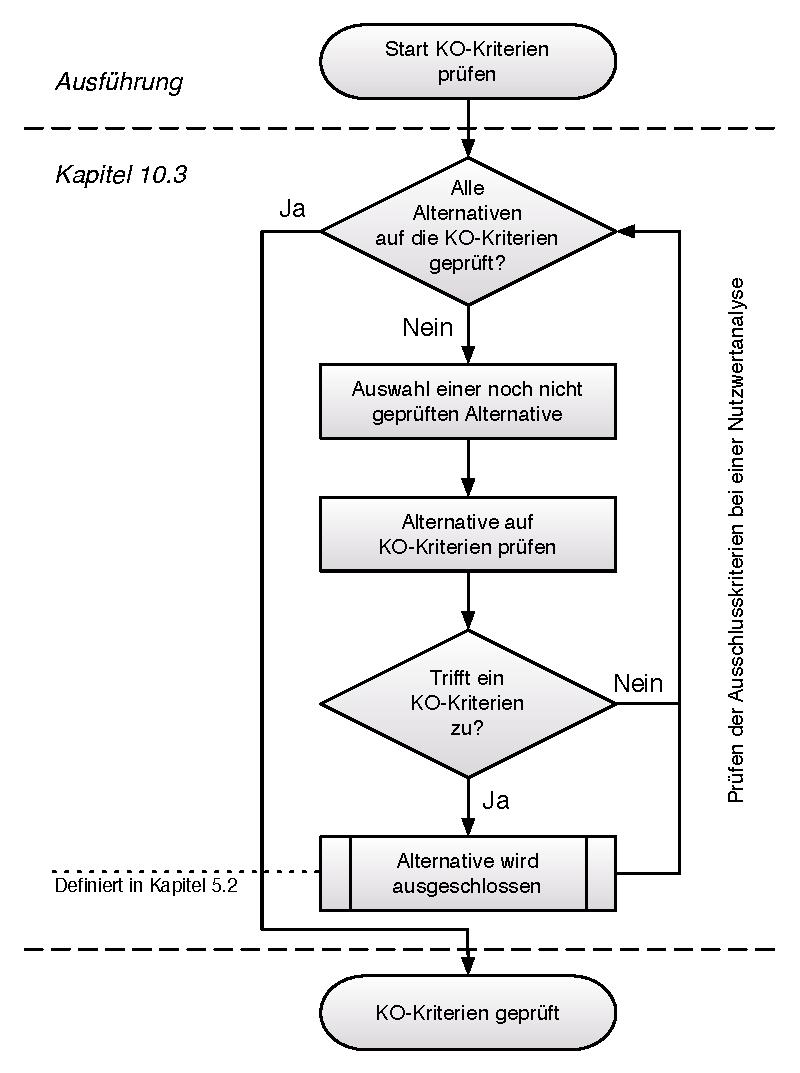
\includegraphics[width=0.7\textwidth]{./image/rahmenbedingungenPruefen.pdf}
      \caption{Die Alternativen sollen gegen KO-Kriterien geprüft werden.}
      \label{img:rahmenbedingungenPruefen}
    \end{center}
  \end{figure}
  
  \clearpage
 
  \section{Analytic Hierarchy Process}
  
  Der Analytic Hierarchy Process stamt aus der Feder eines Mathematikers. Aus
  diesem Grund ist das Verfahren auch einiges Anspruchsvoller als eine
  gewichtete Nutzwertanalyse. Ich gehe hier nicht auf die ganzen Details ein, da
  es den Rahmen der Diplomarbeit übersteigen würde. Totzdem soll eine grober
  Überblick über den \ac{AHP} gegeben werden.
  
  Der \ac{AHP} besteht aus drei Phasen, siehe \cite{AnalyticHierarchyProcess}: 
  
  \begin{enumerate}
    \item Sammeln der Daten
    \item Daten vergleichen und gewichten
    \item Daten verarbeiten
  \end{enumerate}
  
  \subsection{Sammeln der Daten}
  
  In der ersten Phase sollen alle Daten, die für eine Entscheidungsfindung
  erheblich sind, gesammelt werden.
  
  \begin{itemize}
    \item Zuerst soll eine konkrete Frage formuliert werden, für welche die
    beste Antwort gesucht wird.
    \item Danach sollen zu der gestellten Frage alle Kriterien  gesucht werden,
    welche die Lösung beeinflussen können.
    \item Als letztes sollen alle Alternativen gesucht werden, welche als
    mögliche Lösung infrage kommen.
  \end{itemize}
  
  \subsection{Daten vergleichen und gewichten}
  
  In der zweiten Phase folgt nun die Gegenüberstellung, Vergleich und Bewertung
  aller Kriterien beziehungsweise Alternativen in zwei Unterschritten.
  
  \begin{itemize}
    \item Jedes Kriterium wird jedem anderen gegenübergestellt und darauf
    verlgichen, was eine grössere Bedeutung in der gestellten Frage hat. Die
    Skala geht von 1 bis 9, siehe Tabelle \ref{tab:vergleichsgrade}.
    \item Für jedes Kriterium wird jede mögliche Alternativen mit jeder anderen
    gegenübergestellt und auf ihre Eignung hin untersuchen, welche Alternative
    am besten zur Erfüllung des jeweiligen Kriteriums passt. Die Skala geht von
    1 bis 9, siehe Tabelle \ref{tab:vergleichsgrade}.
  \end{itemize}
  
  \begin{table}[ht]
    \sffamily 
    \begin{center}
      \begin{tabular}{lc}
        \toprule
        \textbf{Bedeutung} & \textbf{Skala}\\
        \midrule
        gleiche Bedeutung & 1\\
        leicht grössere Bedeutung & 2 - 3\\
        viel grössere Bedeutung & 4 - 6\\
        erheblich grössere Bedeutung & 7 - 8\\
        absolut dominierend & 9\\
        \bottomrule
      \end{tabular}
      \caption{Skala der Vergleichsgrade}
      \label{tab:vergleichsgrade}
    \end{center}
  \end{table}
    
  \subsection{Daten verarbeiten}
  
  Mit einem mathematischen Modell, kann der \ac{AHP} nun eine präzise Gewichtung
  aller Kriterien errechnen. Mit der Gewichtung der Kriterien und dem Vergleich
  der Alternativen, kann der \ac{AHP} nun berechnen, welches die beste Lösung
  (Alternative) für die gestellt Frage ist. Aus dem mathematischen Modell
  heraus, kann nun ein Inkonsistenzfaktor errechnet werden, der eine Aussage
  macht, wie logisch die Bewertungen zueinander sind.
  
  Diese Berechnungen werden meistens mit der Unterstütztung einer Software
  gemacht. Als Beispiel gibt es JAHP 2.1\footnote{Für Hintergrundinformationen
  zum JAHP 2.1, siehe \cite{JAHP}}, dies ist ein Java Programm mit dem der
  gesammte Prozess des \ac{AHP} abgebildet und berechnet werden kann. Das
  Programm wird unter den Bedingungen der GNU General Public License
  vertrieben.
    
  \section{Kombination beider Methoden}
  
  Diese beiden Methoden können auch kombiniert eingesetzt werden, siehe
  \cite{AhpNwaKombination}, da der \ac{AHP} relativ komplex in der Umsetztung
  ist. Als Kombination kann die Nutzwertanalyse als Methode verwendet werden,
  und der \ac{AHP} wird für die präzise Berechnung der Gewichtung einzelner
  Entscheidungskriterien verwendet. Aus der Kombination entsteht somit eine
  neue Methode, welche durch die Verständlichkeit der \ac{NWA} und der
  objektiven Gewichtung des \ac{AHP} eine plausable Evaluation ermöglicht.

  \subsection{Verbesserung der 
  Gewichtung}\label{subsection:VerbesserungDerGewichtung}
  
  Damit die Gewichtung noch präziser bestimmt werden kann, gibt es verschiedene
  Ansätze. Zwei Ansätze möchte ich hier erläutern:
  
  \begin{itemize}
    \item Die Sensitivitätsanalyse, siehe \cite{Sensitivitaetsanalyse}.
    
    Dabei wird ein einzelner Werte in der Gewichtung gezielt verändert, und das
    Resultat wird danach geprüft. Bei der Methode des \ac{AHP} könnte zum
    Beispiel der Inkonsistenzfaktor geprüft werden, wenn dieser sich Positiv
    verändert, dann zeigt das eine Vergesserung der Gewichtung. Das Vorgehen
    wird iterativ, bis zur Unterschreitung einer definierten Schwelle des
    Inkonsistenzfaktors, fortgeführt.
    
    \item Statistische Methoden, wie der Mittelwert oder der Median, siehe
    \cite{Median} und \cite{Mittelwert}.
    
    Dabei wird der Prozess der Gewichtung von mehr als einer Person
    durchgeführt. Das Ergebniss wird aufgrund der statistischen Methoden
    normalisiert, was zu einem objektiveren Resultat führen wird.
  \end{itemize}
  
  Diese Ansätze zur Verbesserung der Gewichtung werden im Rahmen der
  Diplomarbeit nicht durchgeführt, sollen aber bei einer weiteren Anwendung
  nicht ausgeschlossen werden.
  
  \section{Integration in die IT-Infrastruktur prüfen}
  
  Damit ein Java Web Framework in der IT-Infrastruktur betrieben werden kann,
  muss es deren Ansprüchen genügen. Es soll in einer Analysephase die
  IT-Infrastruktur untersucht werden. Es soll analysiert werden, welche Version
  des \ac{JRE} zur Verfügung gestellt wird, zusätzlich sollen die eingesetzten
  Serverkomponenten veranschaulicht werden. Ein Augenmerk soll auch auf
  eingesetzte Protokolle für die Kommunikation, sowie auf die vorgegebene
  logische und physische Trennung von Schichten in der Serverinfrastruktur
  gelegt werden.
  
  Wenn die Auswahl der zu evaluierenden Java Web Frameworks getroffen wurde,
  soll aufgrund der analysierten IT-Infrastruktur geprüft werden, ob ein Betrieb
  möglich ist. Falls der Betrieb nicht möglich wäre, würde das Java Web
  Framework aus der Evaluation ausgeschlossen werden.
  
  \section{Abdeckung der GUI-Komponenten und Paradigmen}
  
  Da die Evaluation gemacht wird, um bestehende Java Swing Applikationen
  abzulösen, soll auch ein Fokus auf das \ac{GUI} gelegt werden. Im Kapitel
  \ref{chapter:MethodenZurAnalyseVonJavaSwingApplikationen}
  (\nameref{chapter:MethodenZurAnalyseVonJavaSwingApplikationen}, S.
  \pageref{chapter:MethodenZurAnalyseVonJavaSwingApplikationen}ff) wird
  beschrieben, wie besetehende Java Swing Applikationen analysiert werden
  können. Das daraus resultierende Ergebnis soll als Grundlage für die Prüfung
  der Abdeckung der GUI-Komponenten und Paradigmen dienen.
  
  Die Prüfung der Abdeckung zielt darauf ab, herauszufinden, ob eine
  Implementierung mit dem zu evaluierenden Java Web Framework, sinnvoll machbar
  ist. Dabei werden alle erkannten GUI-Komponenten und GUI-Paradigmen der
  analysierten Java Swing Applikationen genommen und mit der Dokumentation des
  zu evaluierenden Java Web Frameworks verglichen. Im diesem Vergleich soll
  festgestellt werden, ob eine Komponente oder ein Pardigma äquivalent
  umsetzbar ist. Der Vergleich findet für jede Komponente und jedes
  Paradigma statt und soll schlussendlich in der Form einer prozentualen
  Abdeckung dokumentiert werden.
  
  Die jeweiligen Prozentangaben berechnen sich wie in den beiden Formeln
  \ref{eq:AbdeckungGuiKomponenten} und \ref{eq:AbdeckungGuiParadigmen}
  dargestellt.

  \begin{equation}
    \label{eq:AbdeckungGuiKomponenten}
    Abdeckung\;GUI\;Komponenten = \frac
    	{gefundene\;GUI\;Komponenten}
    	{mögliche\;GUI\;Komponenten} * 100
  \end{equation}

  \begin{equation}
    \label{eq:AbdeckungGuiParadigmen}
    Abdeckung\;GUI\;Paradigmen = \frac
    	{gefundene\;GUI\;Paradigmen}
    	{mögliche\;GUI\;Paradigmen} * 100
  \end{equation}
  
  Als Voraussetzung, das sich das Java Web Framework für eine mögliche Ablösung
  eignet, soll eine Mindestabdeckung von 80\% aller Komponenten und
  Paradigmen erreicht werden. Diese Schwelle ist verhandelbar und wurde in
  diesem Fall aufgrund des Paretoprinzips\footnote{Das Paretoprinzip, auch
  80-zu-20-Regel, besagt, dass 80\% der Ergebnisse in 20\% der Gesamtzeit eines
  Projekts erreicht werden. Die verbleibenden 20\% der Ergebnisse verursachen
  die meiste Arbeit, siehe \cite{Paretoprinzip}.} gewählt. Der Gedanke dahinter
  ist, dass in einem möglichen Projekt zur Ablösung von einer Java Swing
  Applikation mit dem zu evaluierenden Java Web Framework, in 20\% der Zeit die
  meisten Views äquivalent implementiert werden können. Für die eventuell
  fehlenden GUI-Komponenten oder GUI-Paradigmen sollte dann genügend Zeit zur
  Verfügung stehen, um einen Workaround in der Implementierung auszuarbeiten.
  
  Ob eine Schwelle von 80\% genügend ist, sei dahingestellt, dies sollte in
  einer weiteren Anwendung dieser Methode neu geprüft werden. In der Anwendung
  im Rahmen dieser Diplomarbeit wird ein Java Web Framework, welches eine
  Abdeckung von weniger als 80\% hat, aus der Evaluation ausgeschlossen.
  
  Natürlich wird auf eine möglichst hohe Gesamtabdeckung abgezielt. Wenn zwei
  Java Web Frameworks den selben Nutzwert ausweisen, soll das Framework mit der
  höheren Gesamtabdeckung der GUI-Komponenten und Paradigmen präferiert werden.
  Die Gesamtabdeckung berechnet sich wird wie in der Formel
  \ref{eq:AbdeckungGuiTotal} dargestellt.
  
  \begin{equation}
    \label{eq:AbdeckungGuiTotal}
    Gesamtabdeckung = \frac
    	{gefundene\;Komponenten}
    	{mögliche\;Komponenten} * 100
  \end{equation} 

  
  
  \section{Proof of Concept}
    
  \section{Ablauf einer Evaluation}
  
  In der Abbildung \ref{img:ablaufEvaluation} ist der komplette Ablauf einer
  Evaluation mit der kombinierten Methode aus Nutzwertanalyse und
  \ac{AHP} ersichtlich.
  
  \begin{figure}[h!]
    \begin{center}
      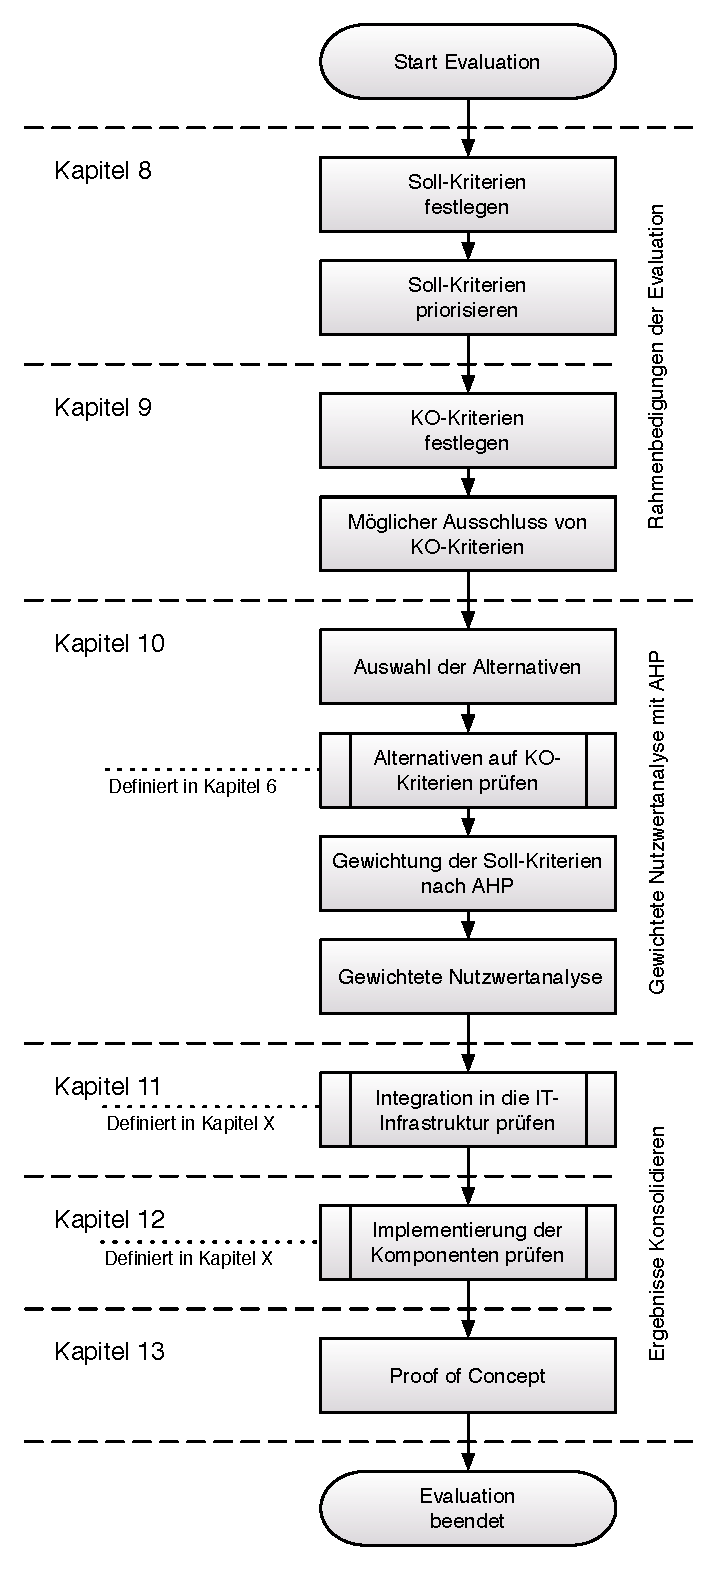
\includegraphics[width=0.7\textwidth]{./image/kompletterAblaufDerEvaluation.pdf}
      \caption{Ablauf einer Evaluation mit der kombinierten Methode aus
      Nutzwertanalyse und \ac{AHP}}
      \label{img:ablaufEvaluation}
    \end{center}
  \end{figure}
